\documentclass{report}
\usepackage{fancyhdr} % Required for custom headers
\usepackage{lastpage} % Required to determine the last page for the footer
\usepackage{extramarks} % Required for headers and footers
\usepackage{graphicx} % Required to insert images
%\usepackage{lipsum} % Used for inserting dummy 'Lorem ipsum' text into the template
\usepackage{amsmath}
\usepackage{graphicx} 
\usepackage{float}
%\usepackage{amsfont}
%\usepackage{amssymb}

\usepackage{multicol}
% Margins
\topmargin=-0.5in
\evensidemargin=0in
\oddsidemargin=-0.5in
\textwidth=7.5in
\textheight=9.0in
\headsep=0.25in 


\pagestyle{fancy}

%\rhead{\textbf{Marshall's Recipes}} % Top right header
%\lhead{\textbf{Curry Stir Fry}}
%\chead{ }
%\title{Curry Stir Fry}

\begin{document}
%\vspace{8mm}
%\textbf{PRELIMINARIES:}


\bigskip

\bigskip

\begin{multicols}{2}
\textbf{Ingredients}
\begin{itemize}
\item 1 cup sliced almonds \newline (480 kCal / 18 gP / 42 gF / 18 gC)
\item $\frac{1}{3}$ cup of olive oil \quad (635 kCal/ 0 gP/ 75 gF/ 0 gC)
\item $\frac{2}{3}$ cup maple syrup \quad (587 kCal/ 0 gP/ 0 gF/ 144 gC)
\item 3 cups rolled oats \quad (900 kCal/ 30 gP/ 15 gF/ 162 gC)
\item $\frac{2}{3}$ cup of unsweetened coconut flakes \newline (267 kCal/ 3 gP/ 24 gF/ 11 gC)
\item 1 cup of dried cranberries \newline (400 kCal/ 4 gP/ 0 gF/ 122 gC)
\item $\frac{1}{2}$ cup of unsalted sunflower seeds\newline (400 kCal/ 13 gP/ 34 gF/ 16 gC)
\item $\frac{1}{4}$ cup of honey \quad (258 kCal / 0 gP / 0 gF / 70 gC) 
\item 3 tsp. vanilla extract
\item 3 tsp. ground cinnamon
\item 1 tsp. sea salt (or $\frac{1}{2}$ tsp. iodized salt)



\end{itemize}


\columnbreak
\textbf{Procedure:}
\medskip


\begin{enumerate}
\item Begin by preheating oven to 300 degrees. Grease a half sheet pan with nonstick spray. 

\item Combine the maple syrup, olive oil, sea salt, cinnamon and vanilla extract in a small saucepan. Heat the mixture for 4-5 minutes over medium heat until warm (the coconut oil should be completely melted) but not simmering, whisking until evenly combined. Remove from heat. 

\item In a large mixing bowl, add the oats, almonds, coconut flakes, pecans and sunflower seeds. Drizzle the maple syrup mixture over the dry ingredients. Gently toss until evenly combined.

\item Spread the granola out evenly on the sheet pan and then gently press it down with a spatula. Bake for 25 minutes, then without stirring, rotate pan 180 degrees. Bake for 15-20 more minutes until the granola is lightly golden on top. Transfer the pan to a wire baking rack and let it cool completely. If the granola seems a bit loose when it comes out of the oven, don’t worry, it will dry and harden as it cools.

\item Once the granola has cooled, use your hands to break it up into your desired size of chunks. Then serve and enjoy! Leftover granola can be stored in an airtight container for up to 2 weeks.

\begin{table}[H]
  \begin{center}
    \caption{Macro totals}
    \label{tab:table1}
    \begin{tabular}{c|c|c|c} % <-- Alignments: 1st column left, 2nd middle and 3rd right, with vertical lines in between
      \textbf{Calories} & \textbf{Protein} & \textbf{Fat} & \textbf{Carbs}\\
      \hline
      3,927 kCal & 68 g & 190 g & 543 g\\
    \end{tabular}
  \end{center}
\end{table}
 
\end{enumerate}
\end{multicols}




%\begin{center}
%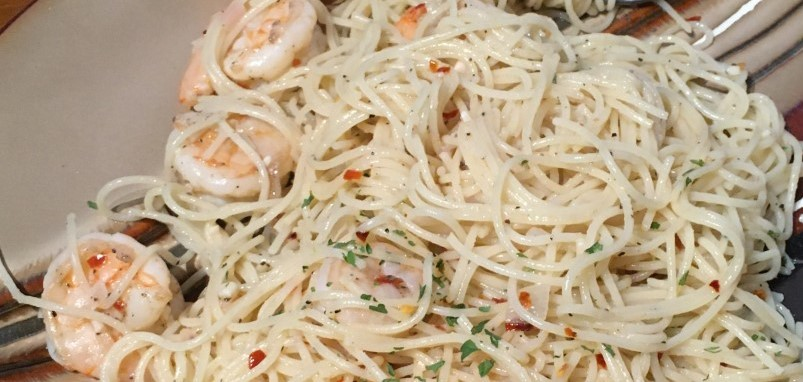
\includegraphics[scale=0.65]{Pasta/Shrimp Scampi/Shrimp Scampi.jpg}
%\end{center}


\end{document}